\documentclass{beamer}
\beamertemplatenavigationsymbolsempty
\graphicspath {{../images/}}

\usepackage[utf8]{inputenc}
\usepackage[czech,english]{babel}
\selectlanguage{czech}

\usepackage{amsmath}
\newcommand{\bra}[1]{\langle#1\rvert} % Bra
\newcommand{\ket}[1]{\lvert#1\rangle} % Ket
\newcommand{\qprod}[2]{ \langle #1 | #2 \rangle} %Inner Product
\newcommand{\braopket}[3]{\langle #1 | #2 | #3\rangle} % Matrix Element
\newcommand{\expect}[1]{ \langle #1 \rangle} % Expectation value
\newcommand\abs[1]{\left|#1\right|}

% Theme
\usetheme{Boadilla}

% Title page
\title{Optimalizácia variačných kvantových eigensolverov}
\author{Michal Švec}
\institute{doc. RNDr. Martin Plesch, PhD.}
\date{December 6, 2023}

\makeatother
\setbeamertemplate{footline}
{
  \leavevmode%
  \hbox{%
  \begin{beamercolorbox}[wd=.3\paperwidth,ht=2.25ex,dp=1ex,center]{author in head/foot}%
    \usebeamerfont{author in head/foot}\insertshortauthor
  \end{beamercolorbox}%
  \begin{beamercolorbox}[wd=.6\paperwidth,ht=2.25ex,dp=1ex,center]{title in head/foot}%
    \usebeamerfont{title in head/foot}\insertshorttitle
  \end{beamercolorbox}%
  \begin{beamercolorbox}[wd=.1\paperwidth,ht=2.25ex,dp=1ex,center]{date in head/foot}%
    \insertframenumber{} /\inserttotalframenumber\hspace*{1ex}
  \end{beamercolorbox}}%
  \vskip0pt%
}
\makeatletter
\setbeamertemplate{navigation symbols}{}
\setbeamertemplate{itemize items}[circle]
\setbeamertemplate{caption}{\raggedright\insertcaption\par}



% Begin document
\begin{document}

% Title slide
\begin{frame}
	\titlepage
\end{frame}

\begin{frame}
	\frametitle{Kvantové počítače}
			
	\begin{columns}[t]
		\begin{column}{.6\textwidth}
			\centering				      
			\begin{itemize}
				\item riadia sa zákonmi kvantovej mechaniky
				\item \begin{itemize} opisuje správanie mirkoskopických systémov ako fotóny, elektróny, atómy, molekuly...\end{itemize}
				\item pravdepodobnostný výpočtový model
				\item využitie paralelizmu
				\item niektoré problémy dokážu vyriešiť rýchlejšie ako štandardné počítače
				\item v súčasnosti ešte nie sú veľmi užitočné \begin{itemize}
				\item najväčší problém predstavuje šum a malý počet qubitov
			\end{itemize}
			\item -273.15°C (0K)
			\end{itemize}
		\end{column}
						      
		\begin{column}{.4\textwidth}
			\centering
									          
			\begin{figure}
				\centering
				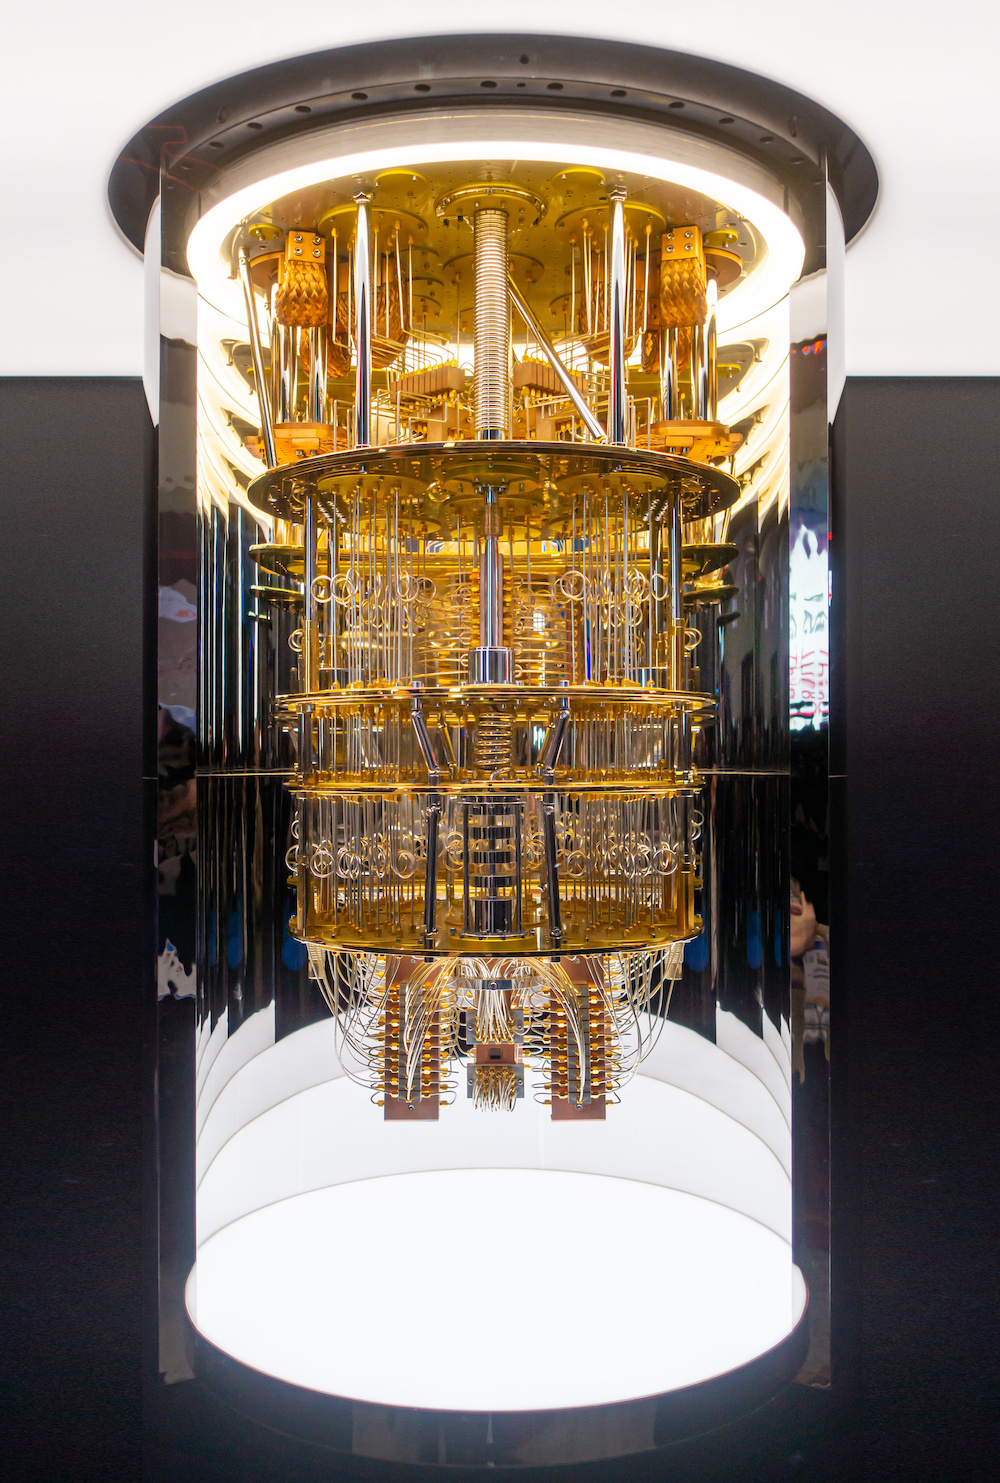
\includegraphics[width=1\textwidth]{quantum_computer.jpeg}            
			\end{figure}
		\end{column}
	\end{columns}
			
			
			
\end{frame}

\begin{frame}
	\frametitle{Bit vs. kvantový bit}
	\begin{columns}[t]
		\begin{column}{.5\textwidth}
			\centering
			Bit (\textbf{b}inary dig\textbf{it})  
			\vspace{0.4cm} 
			\begin{itemize}
				\item najmenšia jednotka informácie v štandardnom počítači
				\item môže byť v dvoch rôznych stavoch, $0$ a $1$
				\item stav sa po meraní nezmení
				\item môžeme kopírovať
				\item booleovská algebra
				      				      
			\end{itemize}
		\end{column}
						      
		\begin{column}{.5\textwidth}
			\centering
			Qubit (quantum bit)
			\vspace{0.4cm}
			\begin{itemize}
				\item najmenšia jednotka informácie v kvantovom počítači
				\item môže byť v stave $\ket{0}$, $\ket{1}$ alebo v akomkoľvek stave, ktorý je lineárnou kombináciou dvoch stavov s komplexnými koeficientami
				\item stav sa zmení počas merania na jeden z dvoch stavov $\ket{0}$ alebo $\ket{1}$
				\item nemôžeme kopírovať
				\item lineárna algebra 
				      
			\end{itemize}		
		\end{column}
	\end{columns}
	% \begin{figure}
	% 	\centering
	% 	\includegraphics[width=0.3\textwidth]{bit_vs_qubit.jpg}            
	% \end{figure}
\end{frame}

\begin{frame}
	\frametitle{Reprezentácia qubitov}
	\begin{itemize}
		\item vektory, matice
		\item Blochova sféra
		\item $\ket{\psi} = \begin{pmatrix}
		      \alpha \\
		      \beta
		\end{pmatrix}$, kde  $\alpha$,$\beta \in \mathbb{C}$ a $\abs{\alpha}^2 + \abs{\beta}^2 = 1$ 
		\item $\abs{\alpha}^2$ je pravdepodobnosť, že qubit nameriame v stave $\ket{1}$
		\item $\abs{\beta}^2$ je pravdepodobnosť, že qubit nameriame v stave $\ket{0}$
	\end{itemize}
	\begin{columns}[c]
		\begin{column}{.3\textwidth}
			\centering
			$\ket{0} = \begin{pmatrix}
			1\\
			0
			\end{pmatrix}$
			\begin{figure}
				\centering
				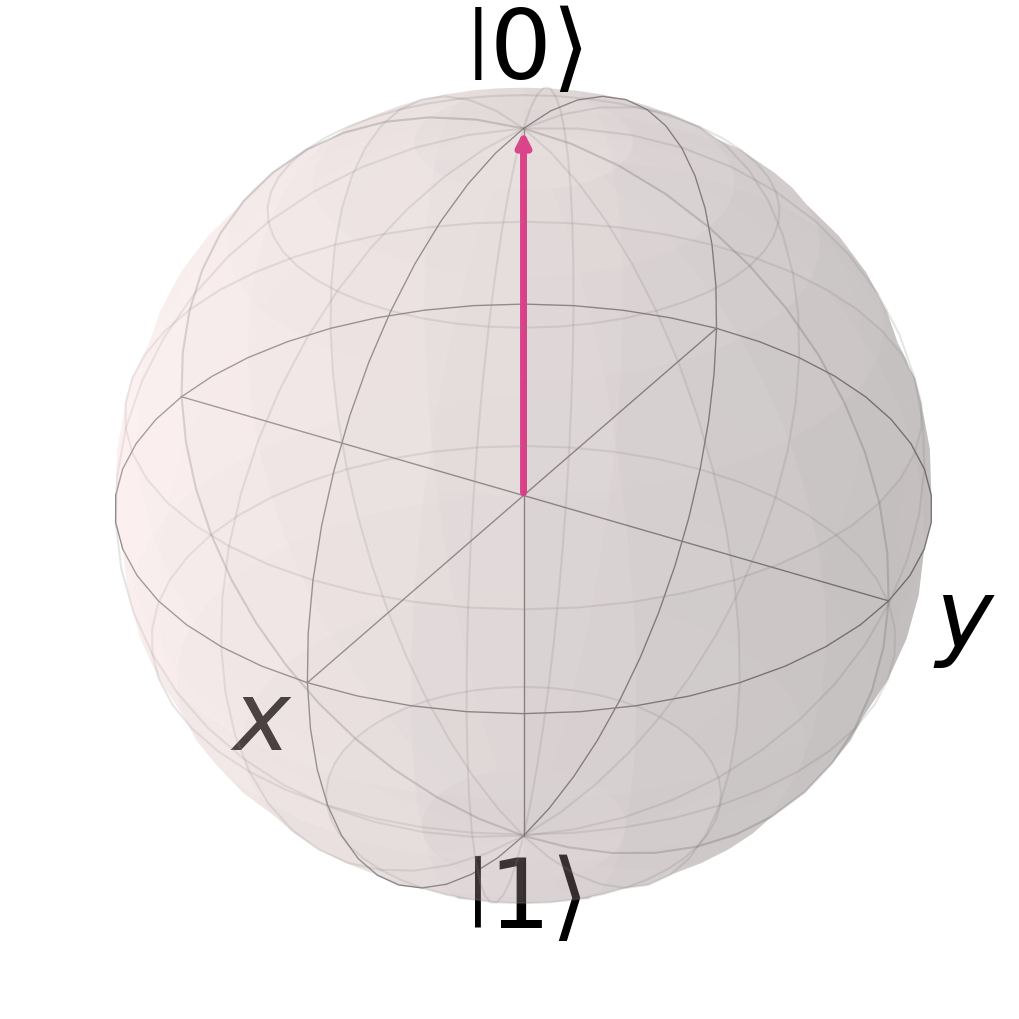
\includegraphics[width=1\textwidth]{qubit0.png}            
			\end{figure}
		\end{column}
						
		\begin{column}{.3\textwidth}
			\centering
			$\ket{1} = \begin{pmatrix}
			0\\
			1
			\end{pmatrix}$
			\begin{figure}
				\centering
				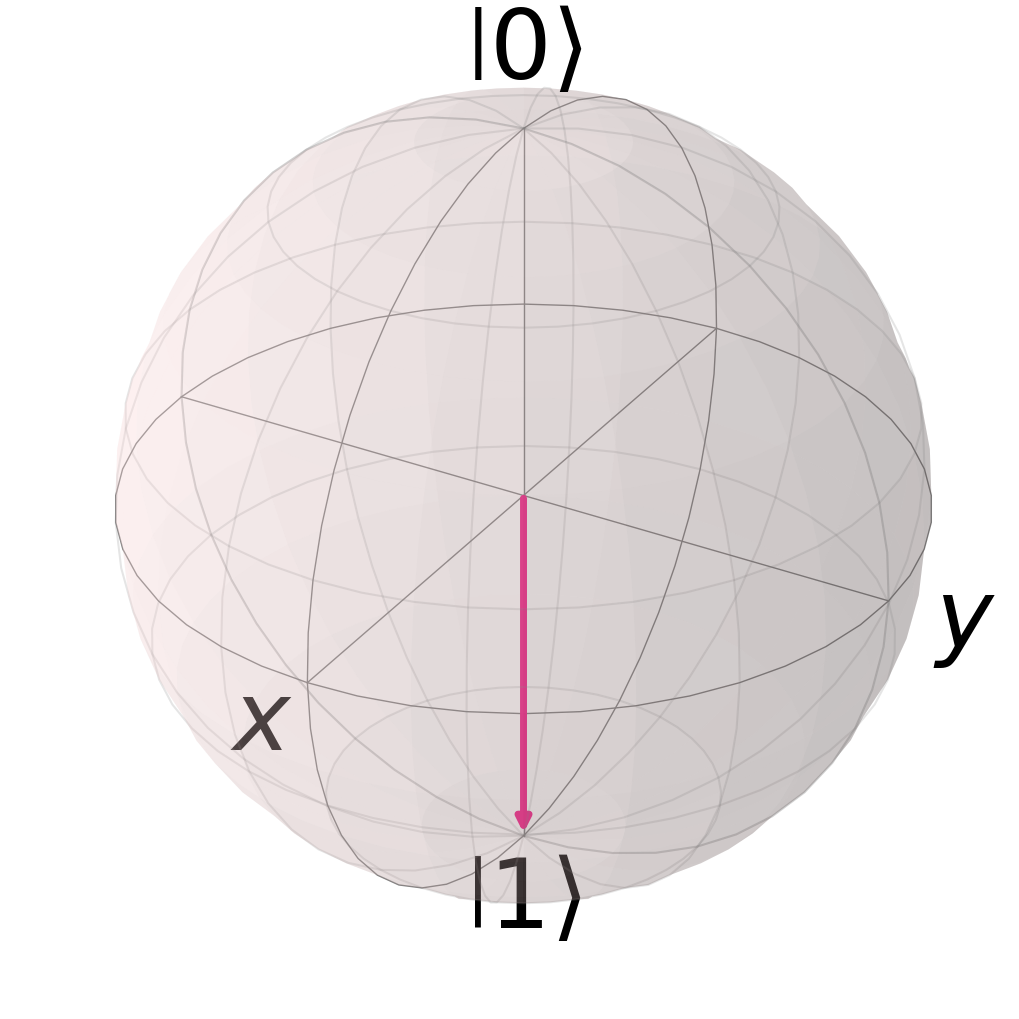
\includegraphics[width=1\textwidth]{qubit1.png}            
			\end{figure}
		\end{column}
						
		
	\end{columns}
			    
\end{frame}

\begin{frame}
	\frametitle{Operácie na bitoch a qubitoch}
	\begin{columns}[t]
		\begin{column}{.5\textwidth}
			\centering
			% first column about standard gates
			Logické hradlá
			\vspace{0.4cm}
			\begin{itemize}
				\item NOT
			\end{itemize}
						     
			\begin{columns}[c]
				% NOT gate image
				\begin{column}{.5\textwidth}
					\begin{figure}
						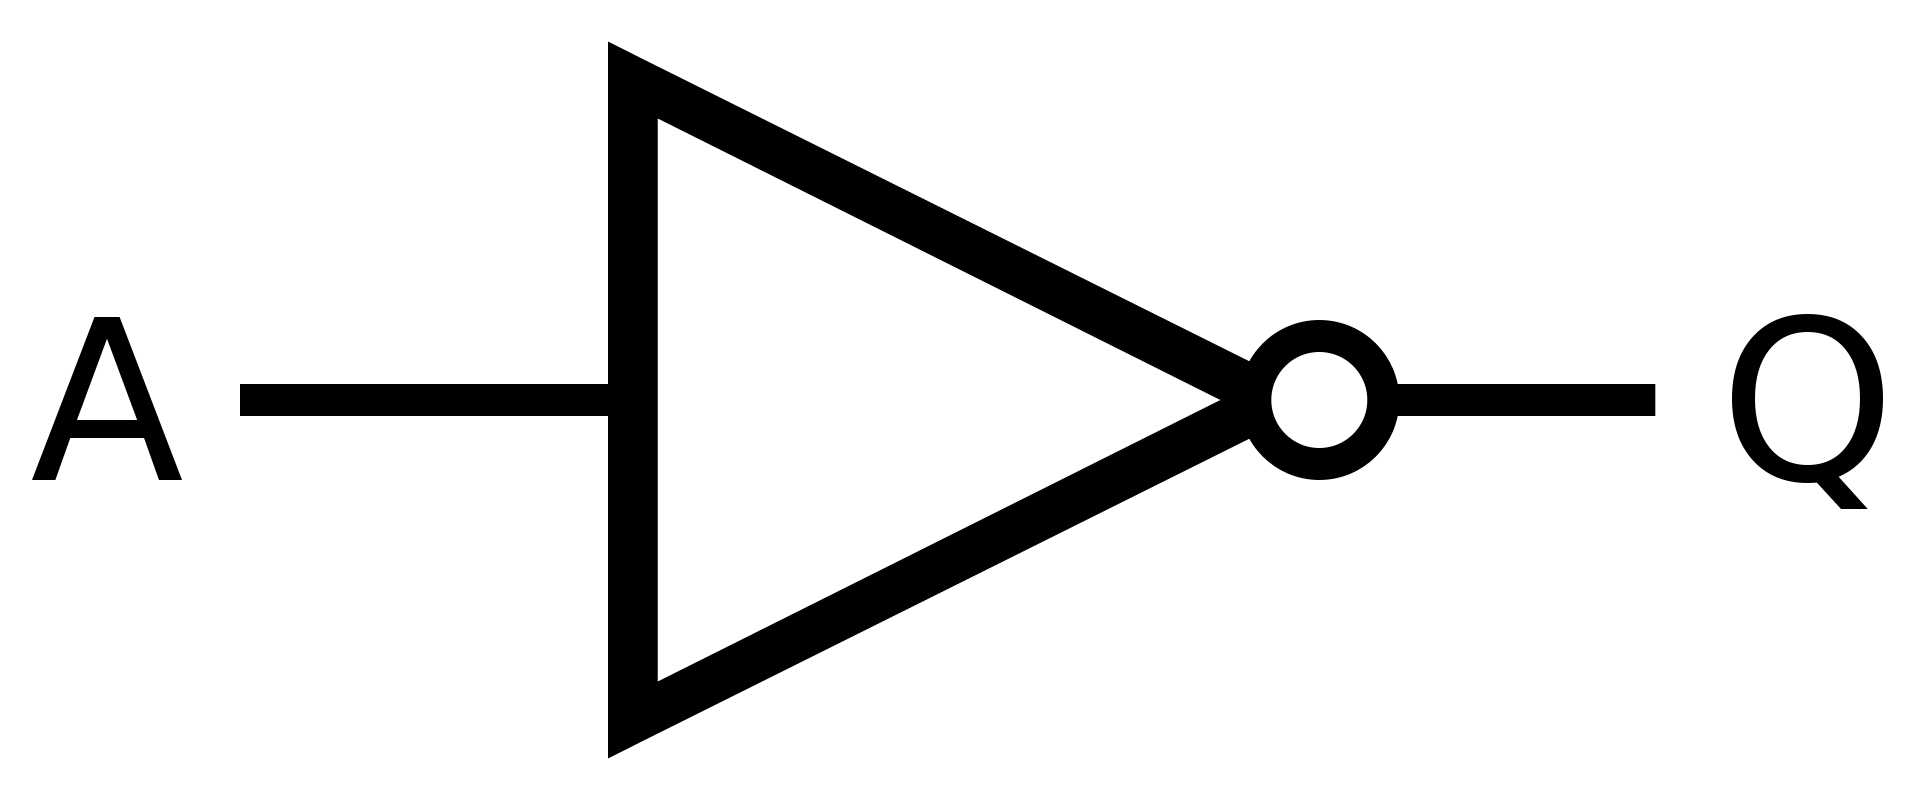
\includegraphics[width=.5\textwidth]{standard_not_gate.png}            
					\end{figure}
				\end{column}
				% NOT gate table
				\begin{column}{.5\textwidth}
					\begin{displaymath}
						\begin{array}{|c|c|}
							\hline
							A & Q \\
							\hline
							0 & 1 \\
							\hline
							1 & 0 \\
							\hline
						\end{array}   
					\end{displaymath}    
				\end{column}
			\end{columns}
			\begin{itemize}
				\item AND
			\end{itemize}
			\begin{columns}[c]
				\begin{column}{.5\textwidth}
					\begin{figure}
						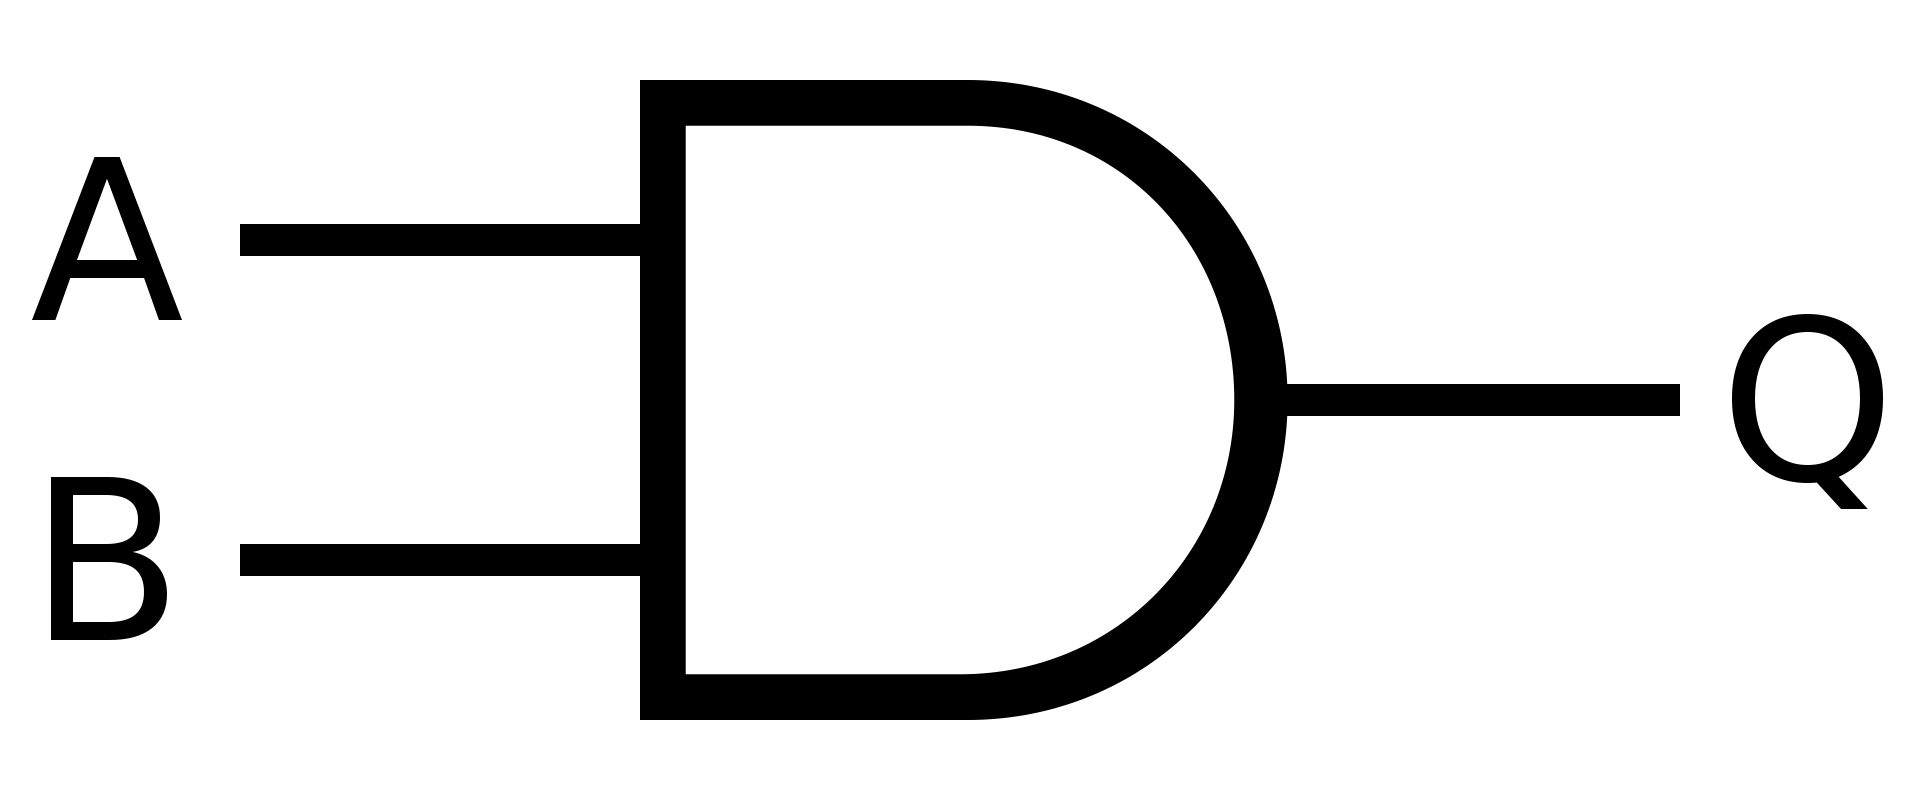
\includegraphics[width=.5\textwidth]{standard_and_gate.png}            
					\end{figure}
				\end{column}
				\begin{column}{.5\textwidth}
					\begin{displaymath}
						\begin{array}{|c c|c|}
							\hline
							A & B & Q \\ 
							\hline 
							0 & 0 & 0 \\
							\hline
							1 & 0 & 0 \\
							\hline
							0 & 1 & 0 \\
							\hline
							1 & 1 & 1 \\
							\hline
						\end{array}   
					\end{displaymath}
				\end{column}
			\end{columns}
			\begin{itemize}
				\item ...
			\end{itemize}
						
		\end{column}
				
		% second column about standard gates
		\begin{column}{.5\textwidth}
			\centering
			Kvantové hradlá
			\vspace{0.4cm}
			\begin{itemize}
				\item Hadamard
			\end{itemize}
								
			\begin{columns}[c]
				% first gate image
				\begin{column}{.5\textwidth}
					\begin{figure}
						\centering
						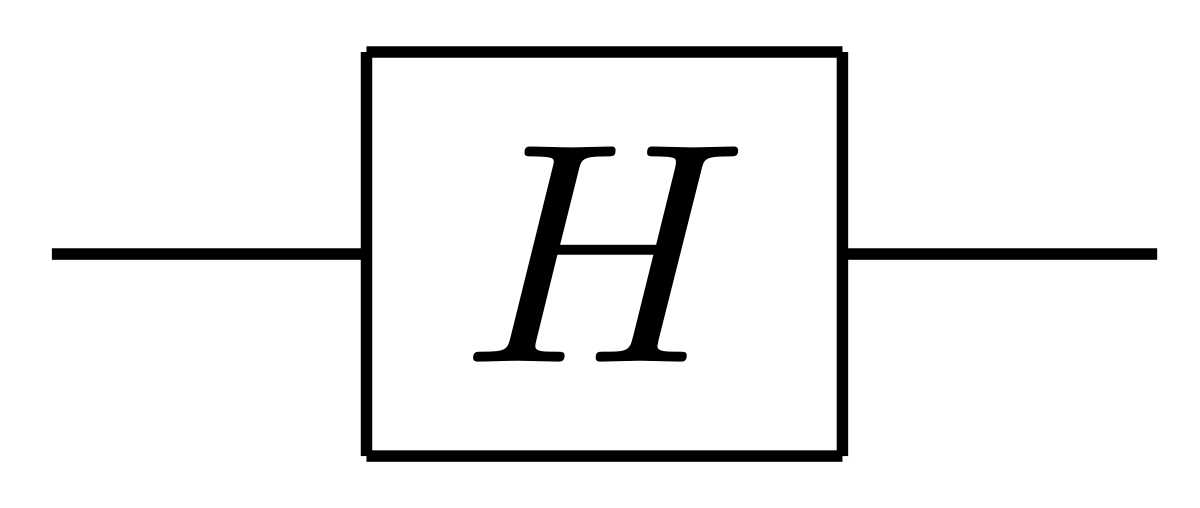
\includegraphics[width=0.5\textwidth]{hadamard_gate.png}
					\end{figure}
				\end{column}
								
				% hadamard gate matrix
				\begin{column}{.5\textwidth}
					$\frac{1}{\sqrt{2}}\begin{pmatrix}
					1 & 1\\
					1 & -1\\
					\end{pmatrix}$
				\end{column}
			\end{columns}  
			\begin{itemize}
				\item Control NOT
			\end{itemize}
							
			\begin{columns}[c]
												
				\begin{column}{.5\textwidth}
					% CNOT gate image
					\begin{figure}
						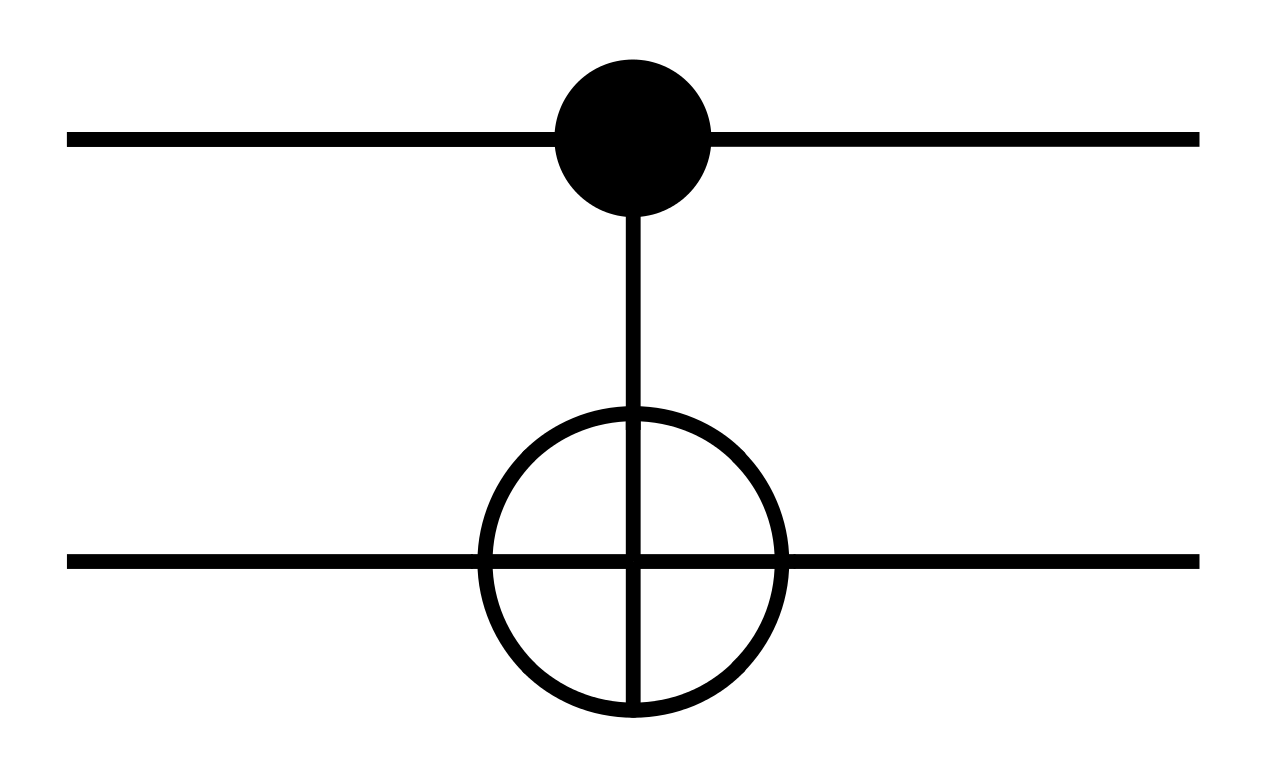
\includegraphics[width=0.5\textwidth]{cnot_gate.png}
					\end{figure}
				\end{column}
				% CNOT gate matrix
				\begin{column}{.5\textwidth}
					$\frac{1}{\sqrt{2}}\begin{pmatrix}
					1 & 0 & 0 & 0\\
					0 & 1 & 0 & 0\\
					0 & 0 & 0 & 1\\
					0 & 0 & 1 & 0\\
					\end{pmatrix}$
				\end{column}
									
			\end{columns}
			\begin{itemize}
				\item ...
				\item všetky hradlá sú reverzibilné
				      				      
			\end{itemize}
		\end{column}
	\end{columns}      
\end{frame}

\begin{frame}[t]
	\frametitle{Superpozícia a kvantové previazanie}
	\begin{columns}[t]
		\begin{column}{.7\textwidth}
			Superpozícia

		\begin{itemize}
			\item stav môže byť lineárnou kombináciou stavov $\ket{0}$ a $\ket{1}$ 
			\begin{itemize}
			\item $\ket{\psi} = \alpha\ket{0} + \beta\ket{1}$
			\item $H\ket{0} = \frac{1}{\sqrt{2}}\ket{0} + \frac{1}{\sqrt{2}}\ket{1} = \begin{pmatrix}
				\frac{1}{\sqrt{2}}\\
				\frac{1}{\sqrt{2}}
				\end{pmatrix}$
		\end{itemize}
				
		\end{itemize}
	\end{column}
		\begin{column}{.3\textwidth}
			\centering
			
			\begin{figure}
				\centering
				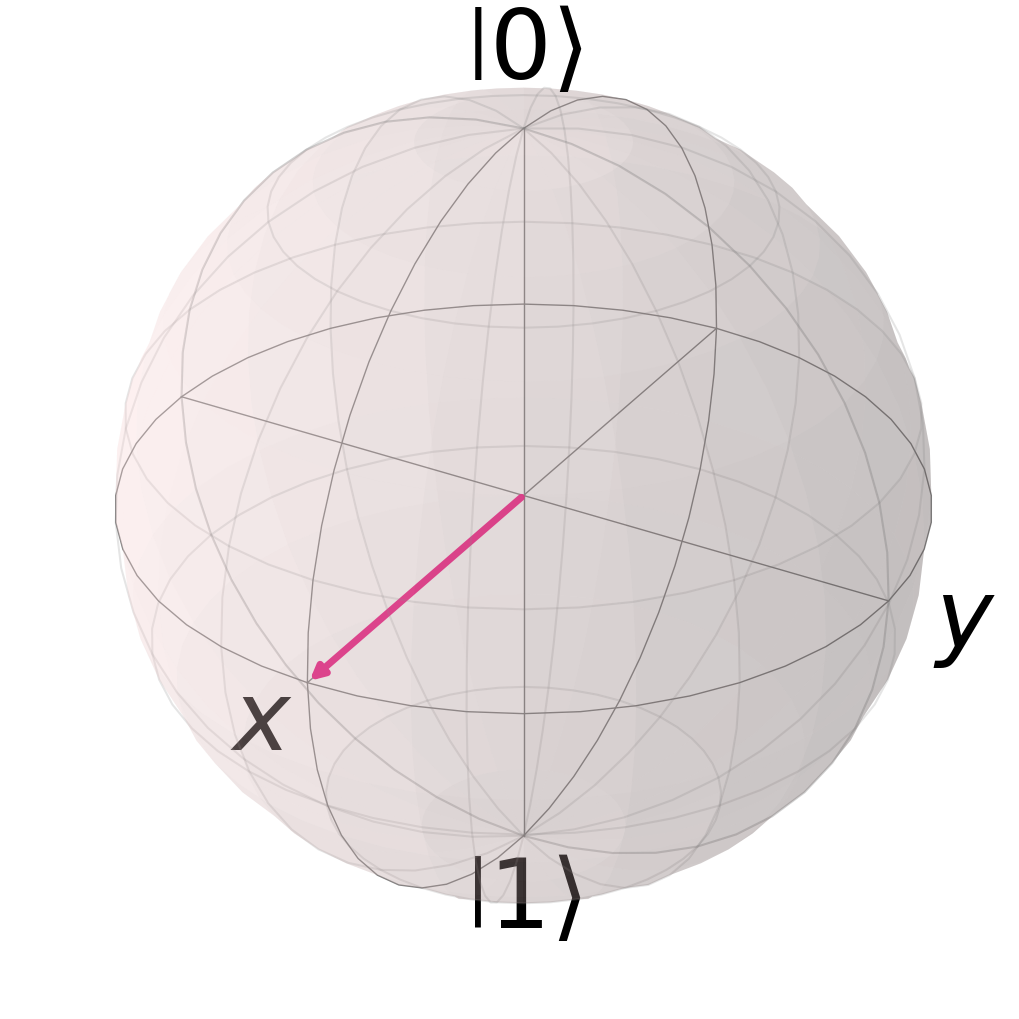
\includegraphics[width=1\textwidth]{qubith.png}            
			\end{figure}
		\end{column}
	\end{columns}
	
	Kvantové previazanie
	\begin{itemize}
		\item stav jedného qubitu je závislý na stave iného qubitu
		\item ľubovoľná vzdialenosť 
		\item $\frac{\ket{00} + \ket{11}}{\sqrt{2}}$		
	\end{itemize}
\end{frame}


\begin{frame}
	\frametitle{Variačný kvantový eigensolver (VQE)}
	\begin{itemize}
		\item hybridný algoritmus
		      \begin {itemize}
		\item súčasne používame štandardný a kvantový počítač
	\end{itemize}
	\item eigensolver
	\item 	\begin{itemize}
	nájde vlastné číslo a vlastný vektor matice
	\end{itemize}
	\item variačný princíp
	\item \begin{itemize}
	umožňuje nájsť zakladný stav systému
	\end{itemize}
	\item jeho hlavné využitie je najmä v chémii
	\begin{itemize} 
		\item nájdenie základného stavu molekuly
	\end{itemize}
	\end{itemize}
			
	\begin{figure}
		\centering
		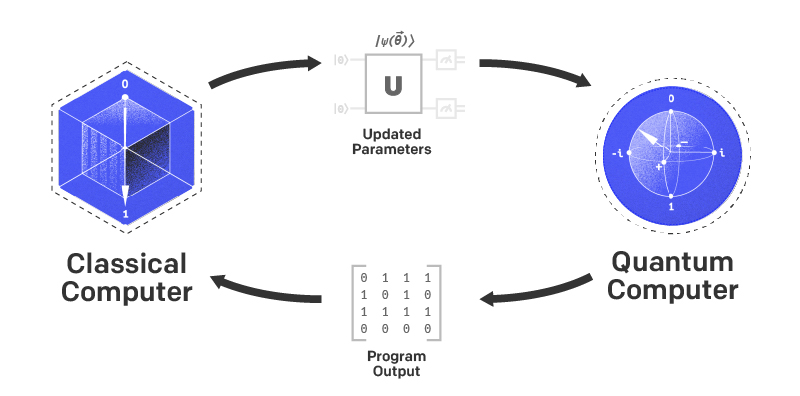
\includegraphics[width=0.75\textwidth]{vqe.jpeg}
		\caption{VQE}
						            
	\end{figure}
\end{frame}


\begin{frame}
	\frametitle{Ciele bakalárskej práce}
	Príprava kvantového stavu
	\begin{itemize}
		\item budeme spúšťať VQE a hľadať najjednoduchšiu prípravu stavu vedúcu k výsledku
		\item pracujeme s knižnicu Qiskit (Quantum Information Science Kit)
		      \begin{itemize}
		      	\item open source Python knižnica vyvíjaná najmä spoločnosťou IBM
		      	\item používame najmä simulátor, skúsime aj skutočný kvantový počítač
		      \end{itemize}
	\end{itemize}
	\begin{figure}
		\centering
		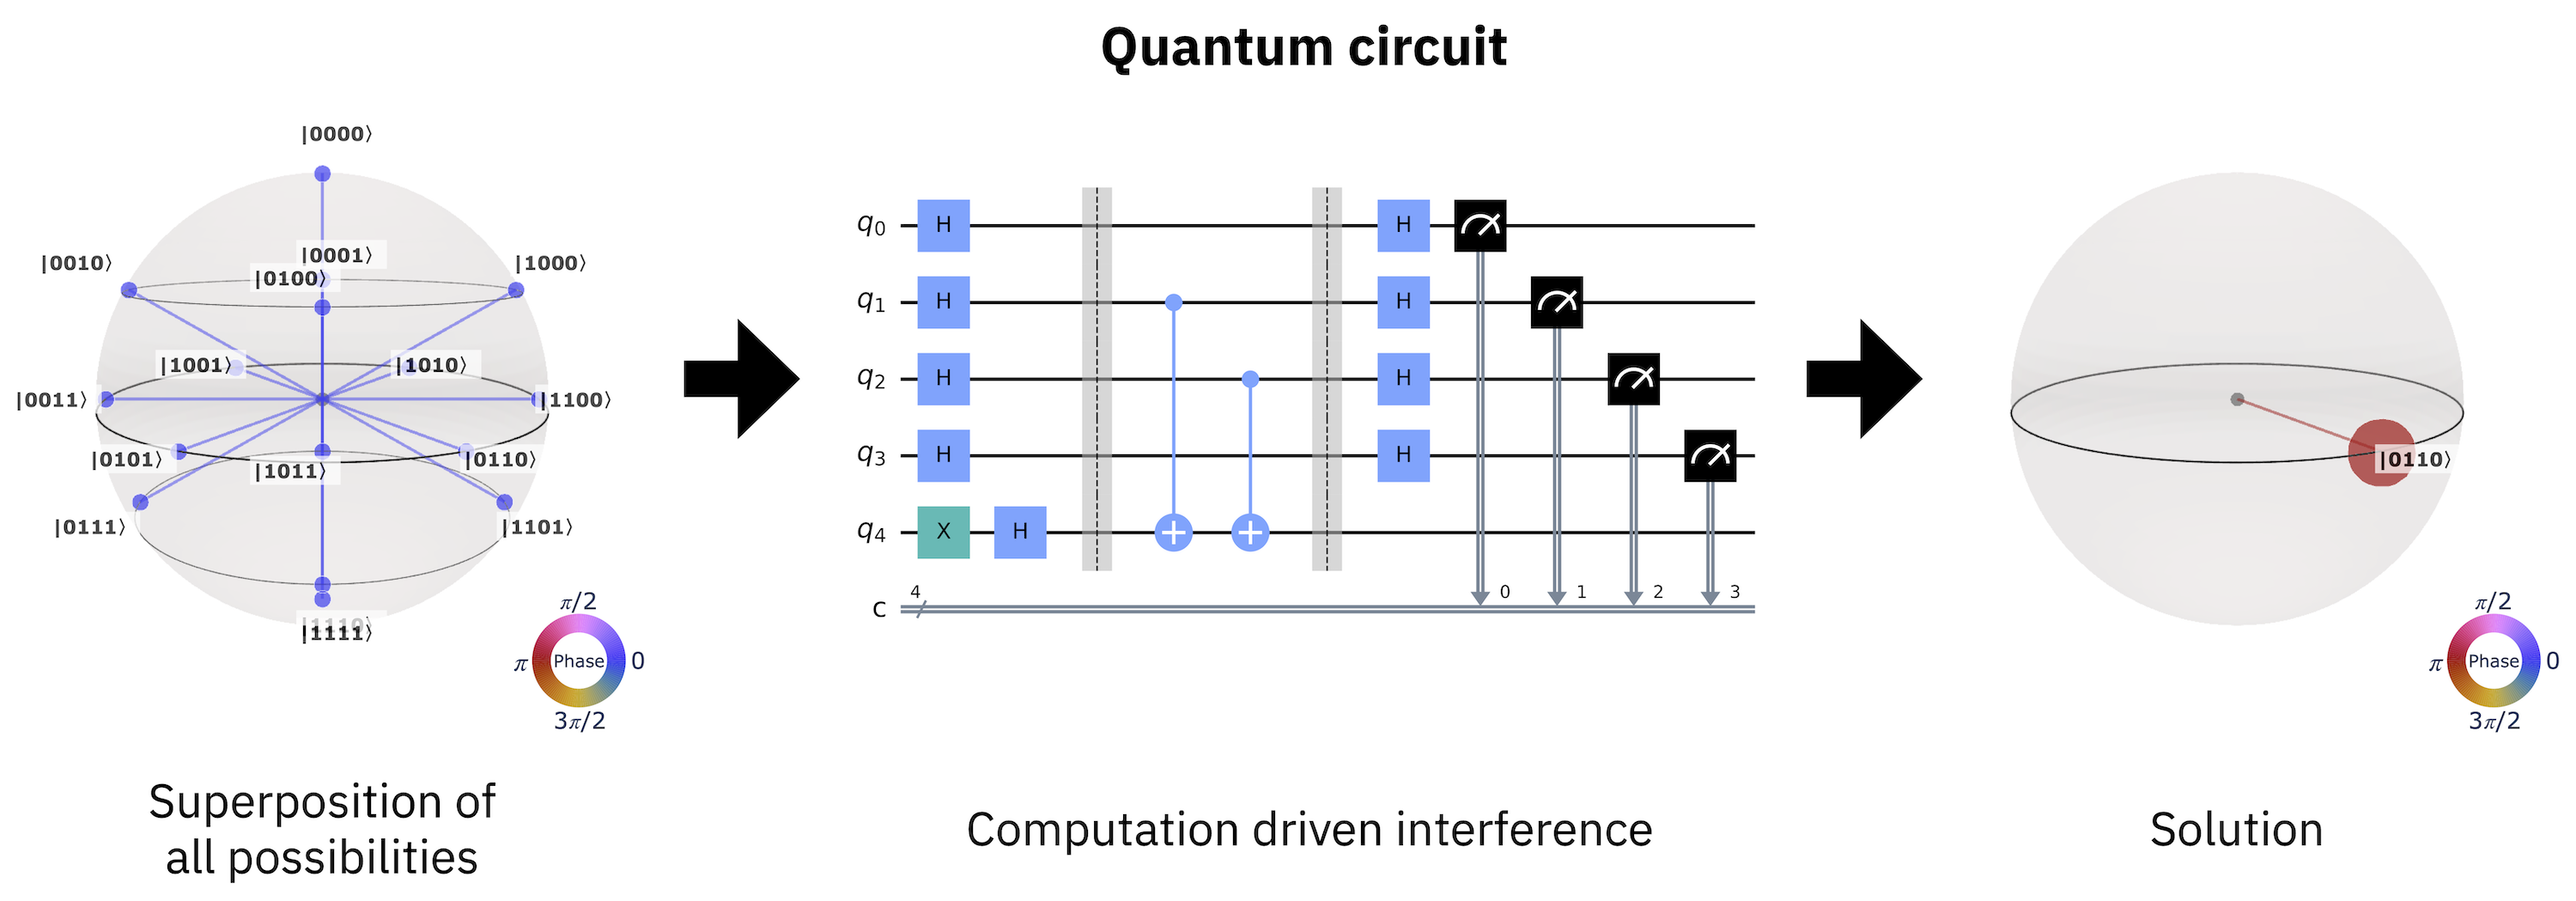
\includegraphics[width=1\textwidth]{quantum_computation.png}
	\end{figure}
\end{frame}

\begin{frame}[t]
	\frametitle{Zdroje}
	\begin{itemize}
		\item \url{https://qiskit.org/documentation/stable/0.34/_images/system_one.jpeg}
		\item \url{https://qiskit.org/documentation/stable/0.40/_images/quantum_interference.png}
		\item \url{https://images.ctfassets.net/hqm865gc1xfs/7ADhfqvgYOEesM5oSFHCiL/eb70f8716e2831015253e1eedced6320/2022-01-06-vqe.jpeg}
	\end{itemize}
\end{frame}
\end{document}